\section{Results}
Table~\ref{tab:main} summarises all models under the four protocols; Fig.~\ref{fig:comparison} visualises the three
RAVDESS-based protocols and the RAVDESS$\to$TESS transfer.

\begin{table*}[t]
\centering
\caption{Accuracy / macro-F1 (\%) on the test sets. Speaker-independent: pooled over all 1,440 clips, $\pm$ is the
standard deviation of accuracy across the 4 speaker folds. Chance (majority class) is 20.0\% on RAVDESS and 14.3\% on
TESS. Bold: best model per protocol, when above chance.}
\label{tab:main}
\begin{tabular}{lccccc}
\toprule
Model & Paper protocol & Aug.-before-split & Speaker-indep. & RAV$\to$TESS & TESS$\to$RAV \\
\midrule
Majority class & 20.1 / 4.8 & 20.0 / 4.8 & 20.0\,$\pm$\,0.0 / 4.8 & 14.3 / 3.6 & 20.0 / 4.8 \\
SVM (RBF) & 77.1 / 76.7 & 85.6 / 85.4 & 49.1\,$\pm$\,4.3 / 48.8 & 23.9 / 17.2 & 13.6 / 7.7 \\
Random Forest & 69.4 / 68.0 & 71.5 / 70.5 & 46.8\,$\pm$\,2.6 / 43.3 & \textbf{31.1 / 23.8} & 14.4 / 5.6 \\
\midrule
1D-CNN & 79.2 / 78.6 & 95.7 / 95.7 & 56.7\,$\pm$\,2.0 / 56.0 & 17.8 / 14.3 & 14.1 / 6.6 \\
CNN\_Bi-LSTM & 81.2 / 80.6 & 94.4 / 94.5 & 56.5\,$\pm$\,2.9 / 56.2 & 17.9 / 17.1 & 13.6 / 4.0 \\
Averaging ensemble & \textbf{81.9 / 81.4} & \textbf{96.5 / 96.6} & \textbf{58.5\,$\pm$\,1.9 / 57.8} & 19.7 / 17.0 & 14.1 / 6.6 \\
\bottomrule
\end{tabular}

\end{table*}

\begin{figure*}[t]
\centering
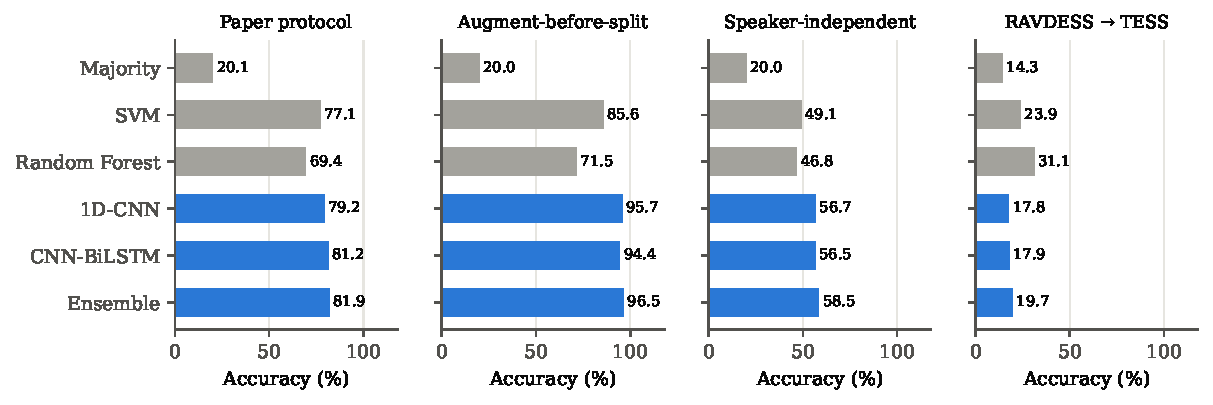
\includegraphics[width=\textwidth]{../results/figures/fig_model_comparison.pdf}
\caption{Accuracy of every model as the protocol becomes stricter (left to right). Grey: classical baselines;
blue: the paper's models. The same ensemble ranges from \AccLeakyEns\% to \AccRTEns\%.}
\label{fig:comparison}
\end{figure*}

\subsection{H1 -- Replication under the paper's protocol}
With augmentation applied to training clips only, our ensemble reaches \AccPaperEns\% accuracy
(weighted F1 \FwPaperEns\%), \ReportedGapEns{} points below the 97.57\% reported (Table~\ref{tab:replication}). The ordering of the
models matches the paper (ensemble $\geq$ CNN\_Bi-LSTM $\geq$ 1D-CNN), and all deep models beat the SVM
(\AccPaperSvm\%) and Random Forest (\AccPaperRf\%). \textbf{H1 is not supported}: the reported figure is not
reproduced under a leak-free split.

\begin{table}[t]
\centering
\caption{RAVDESS replication: accuracy and weighted F1 (\%).}
\label{tab:replication}
\footnotesize\setlength{\tabcolsep}{3pt}
\resizebox{\columnwidth}{!}{\begin{tabular}{lcccccc}
\toprule
 & \multicolumn{2}{c}{Reported in paper} & \multicolumn{2}{c}{Ours: paper protocol} & \multicolumn{2}{c}{Ours: aug.-before-split} \\
\cmidrule(lr){2-3}\cmidrule(lr){4-5}\cmidrule(lr){6-7}
Model & Acc. & W-F1 & Acc. & W-F1 & Acc. & W-F1 \\
\midrule
1D-CNN & 96.18 & 96.22 & 79.17 & 79.04 & 95.66 & 95.65 \\
CNN\_Bi-LSTM & 97.57 & 97.29 & 81.25 & 81.14 & 94.44 & 94.44 \\
Averaging ensemble & 97.57 & 97.56 & 81.94 & 81.94 & 96.53 & 96.53 \\
\bottomrule
\end{tabular}
}
\end{table}

\subsection{H2 -- Augmenting before splitting inflates accuracy}
When the 5,760 augmented samples are pooled \emph{before} the 80/10/10 split, \LeakyOverlap\% of the test samples
have at least one augmented copy of the same recording in the training set. The ensemble then scores
\AccLeakyEns\% (1D-CNN \AccLeakyCnn\%), within about one percentage point of the paper's 97.57\% and 96.18\%.
Accuracy is \LeakyAccOriginal\% on original test clips and \LeakyAccNoisepitch\% on noise+pitch copies, i.e.\ the
model recognises recordings it has effectively already seen. \textbf{H2 is supported}. The paper does not state
the split order, so we cannot prove this is what happened there, but it is the only one of our settings that
reproduces its numbers, and the inflation (+\LeakGainEns{} points for the ensemble) is much larger for the high-capacity deep
models than for the SVM (+\LeakGainSvm), consistent with memorisation of near-duplicates~\cite{kapoor2023leakage}.

\subsection{H3 -- Unseen speakers}
Holding out whole actors lowers ensemble accuracy to \AccSpkEns\,$\pm$\,\AccStdSpkEns\% (macro-F1 \FoneSpkEns\%), a
drop of \SpkDropEns{} points from the paper protocol. The deep models still beat the best classical baseline
(SVM, \AccSpkSvm\%) by \SpkEnsOverSvm{} points, so they do learn transferable cues, but performance varies strongly between
speakers: from \ActorAccMin\% (\ActorMin) to \ActorAccMax\% (\ActorMax). Recall is highest for \SpkRecallMaxName{}
(\SpkRecallMax\%) and lowest for \SpkRecallMinName{} (\SpkRecallMin\%); the most frequent errors are
\ConfOne{} (\ConfOnePct\% of sad clips), \ConfTwo{} (\ConfTwoPct\%) and \ConfThree{} (\ConfThreePct\%)
(Fig.~\ref{fig:confusion}). \textbf{H3 is supported}.

\begin{figure*}[t]
\centering
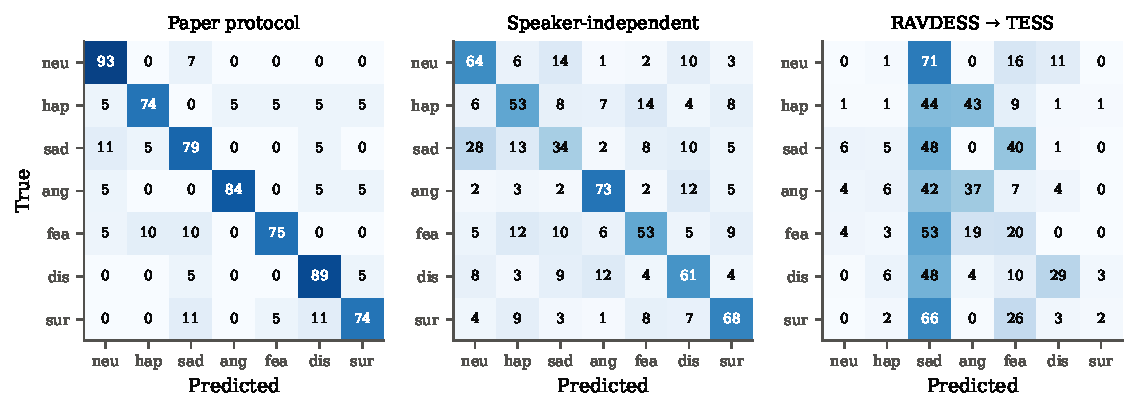
\includegraphics[width=0.92\textwidth]{../results/figures/fig_confusion.pdf}
\caption{Row-normalised confusion matrices (\%) of the ensemble. Under the paper protocol most mass is on the
diagonal; for unseen speakers low-arousal emotions (neutral, sad) are confused; on TESS predictions collapse onto a
few classes.}
\label{fig:confusion}
\end{figure*}

\subsection{H4 -- Unseen dataset}
Cross-corpus transfer fails in both directions. Trained on RAVDESS, the ensemble reaches only \AccRTEns\% on TESS
(chance 14.3\%) and labels \TessTopPredShare\% of all TESS clips as \emph{\TessTopPred}. Trained on TESS, it scores
\AccTREns\% on RAVDESS, \emph{below} the 20.0\% majority baseline, and predicts \emph{\RavTopPred} for
\RavTopPredShare\% of clips. Per-class recall on TESS (RAVDESS-trained ensemble) is:

\smallskip
\centerline{\small\begin{tabular}{ccccccc}
\toprule
Ang. & Dis. & Fea. & Hap. & Neu. & Sad. & Sur. \\
\midrule
37.0 & 29.2 & 20.2 & 0.8 & 0.2 & 48.5 & 2.0 \\
\bottomrule
\end{tabular}
}
\smallskip

\noindent Interestingly, the Random Forest transfers best (\AccRTRf\%). Its time-pooled statistics do not depend
on \emph{where} in the 2.5\,s window a sound occurs, whereas the paper's flattened vector ties every value to a
fixed frame position. \textbf{H4 is supported.}

\paragraph{Controlled check: zero padding.} TESS clips are short, so after the 0.6\,s offset \OffsetPadPaper\% of
TESS frames are zero padding, against \RavPadPct\% for RAVDESS. Silent frames have near-zero energy and look like
low-arousal speech. To test this without retraining, we re-extracted TESS with offset 0\,s
(\OffsetPadZero\% padding) and evaluated the \emph{same} RAVDESS-trained models: accuracy rises from
\OffsetAccPaper\% to \OffsetAccZero\% and the share of ``sad'' predictions falls from \OffsetSadPaper\% to
\OffsetSadZero\%. Padding therefore explains part of the collapse, but even without it the model remains far below
its within-corpus accuracy, pointing to the other differences between corpora: speakers, single words vs.\
sentences, and recording conditions. The older TESS speaker is recognised worse (\TessAccOaf\% vs.\
\TessAccYaf\% for the younger one).

\subsection{H5 -- Gender bias check}
Every model is more accurate for female than for male actors (Table~\ref{tab:gender}, Fig.~\ref{fig:gender}). For
the ensemble the gap is \GenderGapEns{} points (\GenderFemaleEns\% vs.\ \GenderMaleEns\%, $p$\,\GenderPEns{} by a
two-proportion $z$-test). Because clips of the same actor are not independent, we also compared the 24 per-actor
accuracies: the female actors are still clearly better (Mann--Whitney $U=\GenderActorU$ of a maximum 144,
$p=\GenderActorP$). The data are balanced (12 actors and 720 clips per gender), so this is not a sampling artefact
of RAVDESS's composition. The gap is largest for surprised, neutral and disgust and is the only one reversed for
happy (Table~\ref{tab:gender_emotion}). \textbf{H5 is supported}: a model deployed from this pipeline would
systematically serve male speakers worse.

\begin{table}[t]
\centering
\caption{Bias check, speaker-independent protocol (720 clips per gender). Gap = female $-$ male.}
\label{tab:gender}
\footnotesize\setlength{\tabcolsep}{3pt}
\resizebox{\columnwidth}{!}{\begin{tabular}{lccccc}
\toprule
Model & Acc. male & Acc. female & Gap (pp) & $z$ & $p$ \\
\midrule
SVM (RBF) & 45.3 & 52.9 & +7.6 & -2.90 & 0.004 \\
Random Forest & 41.0 & 52.6 & +11.7 & -4.44 & $<$0.001 \\
1D-CNN & 49.4 & 63.9 & +14.4 & -5.53 & $<$0.001 \\
CNN\_Bi-LSTM & 47.2 & 65.8 & +18.6 & -7.12 & $<$0.001 \\
Averaging ensemble & 50.7 & 66.2 & +15.6 & -5.99 & $<$0.001 \\
\bottomrule
\end{tabular}
}
\end{table}

\begin{figure}[t]
\centering
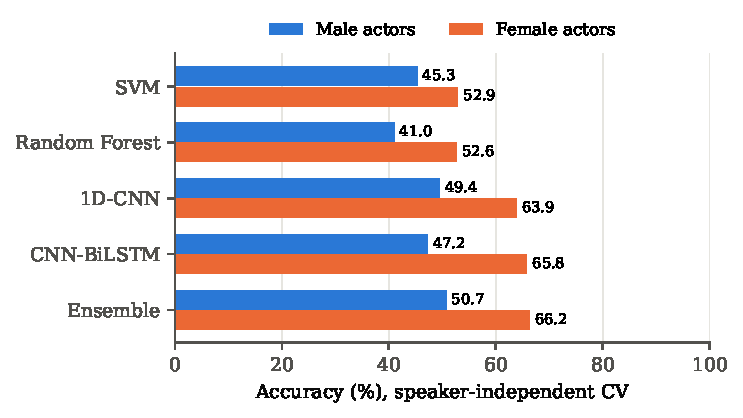
\includegraphics[width=\columnwidth]{../results/figures/fig_gender_bias.pdf}
\caption{Accuracy by speaker gender (speaker-independent CV).}
\label{fig:gender}
\end{figure}

\begin{table}[t]
\centering
\caption{Per-emotion recall (\%) of the ensemble by gender.}
\label{tab:gender_emotion}
\small
\begin{tabular}{lccc}
\toprule
Emotion & Recall male & Recall female & Gap (pp) \\
\midrule
Neutral & 54.2 & 74.3 & +20.1 \\
Happy & 54.2 & 52.1 & -2.1 \\
Sad & 30.2 & 38.5 & +8.3 \\
Angry & 67.7 & 79.2 & +11.5 \\
Fearful & 43.8 & 61.5 & +17.7 \\
Disgust & 51.0 & 70.8 & +19.8 \\
Surprised & 52.1 & 83.3 & +31.2 \\
\bottomrule
\end{tabular}

\end{table}

\subsection{H6 -- Feature and augmentation ablation}
\label{sec:ablation}
Table~\ref{tab:ablation} retrains the 1D-CNN and the SVM on the paper-protocol split with parts of the input removed.
The test set has 144 clips, so one clip is \AblClipPct{} points and the standard error of an accuracy near 79\%
is about \AblSE{} points; differences smaller than roughly twice that are not meaningful.

\begin{table}[t]
\centering
\caption{Ablation on the paper-protocol split (accuracy \%, 144 test clips). $\Delta$ is relative to the full
1D-CNN (79.2\%). *Training stopped at epoch 9 with validation accuracy at chance level (see text).}
\label{tab:ablation}
\footnotesize\setlength{\tabcolsep}{3pt}
\resizebox{\columnwidth}{!}{\begin{tabular}{lcccc}
\toprule
Variant & Input dim. & SVM acc. & 1D-CNN acc. & $\Delta$ CNN (pp) \\
\midrule
All features (ZCR+RMSE+MFCC+Chroma) & 3{,}672 & 77.1 & 79.2 & -- \\
without ZCR & 3{,}564 & 77.1 & 79.9 & +0.7 \\
without RMSE & 3{,}564 & 77.1 & 79.2 & +0.0 \\
without MFCC & 1{,}512 & 45.1 & 56.9 & $-$22.2 \\
without Chroma & 2{,}376 & 79.2 & 73.6 & $-$5.6 \\
MFCC only & 2{,}160 & 78.5 & 80.6 & +1.4 \\
No augmentation (paper early stopping) & 3{,}672 & 78.5 & 31.2 & $-$47.9 \\
No augmentation, patience 20 & 3{,}672 & -- & 74.3 & $-$4.9 \\
\bottomrule
\end{tabular}
}
\end{table}

\begin{itemize}
  \item \textbf{MFCC is essential.} Removing the 20 MFCCs changes accuracy by \AblNomfcc{} points for the 1D-CNN and
        \AblSvmNomfcc{} for the SVM, the only feature removal clearly beyond noise. \emph{MFCC alone}
        (\AblAccMfcconly\%) is at least as accurate as the full feature set.
  \item \textbf{ZCR and RMSE add nothing measurable} ($\Delta$ of \AblNozcr{} and \AblNorms{} points).
  \item \textbf{Chroma: inconsistent.} Removing Chroma changes the 1D-CNN by \AblNochroma{} points but
        the SVM by \AblSvmNochroma{} (opposite directions). Both changes are within about two standard errors, so we find no
        robust evidence for the paper's LIME-based claim that Chroma contributes substantially.
  \item \textbf{Augmentation helps modestly, and interacts with early stopping.} Without augmentation, training
        stops at epoch 9 with validation accuracy still at chance, giving \AblAccNoaugmentation\%. The cause is that an
        un-augmented epoch has 4$\times$ fewer updates (18 vs.\ 72 batches), so the paper's patience of 5 epochs is
        too short. With a patience of 20 epochs, the un-augmented model reaches \AblAccNoaugmentationpatiencetwenty\%,
        so dropping augmentation changes accuracy by \AblNoaugmentationpatiencetwenty{} points (about 1.4 standard
        errors), not \AblNoaugmentation. Augmentation therefore helps modestly at best on this split.
\end{itemize}
\textbf{H6 is partly supported}: MFCC carries almost all the information; a positive contribution of Chroma is not
confirmed. A practical corollary, on this split, is that a 2,160-value MFCC-only input gives a smaller model with no loss in
accuracy.

\begin{figure}[t]
\centering
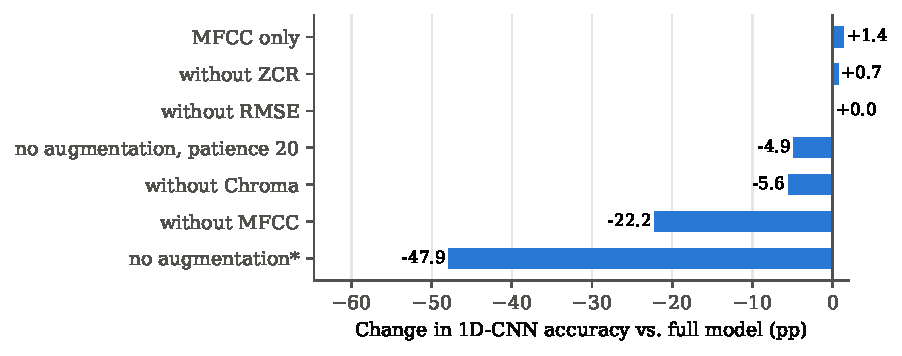
\includegraphics[width=\columnwidth]{../results/figures/fig_ablation.pdf}
\caption{Change in 1D-CNN accuracy when parts of the input are removed (paper-protocol split). *No augmentation
with the paper's early stopping, which halts before the model learns; see text.}
\label{fig:ablation}
\end{figure}


\subsection{Efficiency}
The 1D-CNN has \ParamsCnn{} parameters and the CNN\_Bi-LSTM \ParamsLstm{} (ensemble \ParamsEns{}). On a 4-core CPU,
training under the paper protocol took \FitMinCnn{} and \FitMinLstm{} minutes (\EpochsCnn{} and \EpochsLstm{}
epochs before early stopping), and inference costs \InferMsCnn{} and \InferMsLstm{} ms per clip. The SVM trains in
seconds and predicts in \InferMsSvm{} ms per clip, and it is only \PaperEnsOverSvm{} points behind the ensemble under the paper
protocol, which puts the value of the deep ensemble in perspective.

\section{Error Analysis and Discussion}
\label{sec:discussion}
\paragraph{Why the paper's protocol overestimates performance.} Emotion corpora such as RAVDESS contain a small
number of speakers who each record the same two sentences many times. A random split therefore places recordings of
the \emph{same actor saying the same sentence} in both training and test sets, and augmentation before the split
adds near-copies of the \emph{same recording}. Both violate the assumption that test data are independent of
training data. The 97\% figure measures recognition of familiar voices (or familiar recordings), not of emotion.

\paragraph{Why the models fail on new speakers.} The input is a globally standardised vector of absolute feature
values. MFCC and Chroma levels depend strongly on vocal-tract shape and fundamental frequency, i.e.\ on
\emph{who} is speaking; nothing in the pipeline removes speaker identity, so a model can reach high within-speaker
accuracy by learning speaker-specific baselines. For a new speaker those baselines are wrong. The dominant errors
(\ConfOne, \ConfTwo) are between low-arousal classes whose differences are subtle relative to between-speaker
variation. Merging RAVDESS \emph{calm} into \emph{neutral}, as the paper does, makes the neutral class more
heterogeneous and adds to this confusion.

\paragraph{Why women are recognised better.} We can only offer hypotheses: female voices typically have a higher and
wider pitch range, which Chroma and MFCC capture, so emotional pitch changes may be more separable; and the
augmentation (pitch shift of +0.7 semitones) never moves a voice across the male--female range. Speaker-level
normalisation or gender-balanced model selection would be the first mitigations to test.

\paragraph{Why cross-corpus transfer collapses.} Besides speakers, the corpora differ in utterance type (a full
sentence vs.\ ``Say the word \_\_''), duration (hence padding), speaker age and recording setup. The flattened,
position-dependent representation amplifies these differences: the same emotion expressed 0.3\,s later produces a
different input vector. The controlled padding check shows that one of these factors alone moves accuracy by
\OffsetGain{} points.

\paragraph{Take-away.} The paper's architecture is a reasonable lightweight model: it beats classical baselines under
every within-corpus protocol. But its reported accuracy is a property of the evaluation protocol as much as of the
model. For deployment, the speaker-independent figure (\AccSpkEns\%) and the cross-corpus figure (near chance)
are the relevant ones.
